\section{Theoretische Grundlagen}
\label{sec:Theorie}

\subsection{Das Prinzip der Wärmepumpe}
Betrachtet man zwei Flüssigkeitsreservoire mit den Temperaturen $T_1$ und $T_2$, wobei $T_1 > T_2$ gilt, dann wird solange Wärmeenergie vom Reservoir $1$ zum Reservoir $2$ übertragen, bis die Temperaturdifferenz $\Delta T := T_1 - T_2$ gleich Null ist, also die Temperaturen gleich sind.
Dieser Wärmetransport lässt sich allerdings mit Hilfe einer Wärmepumpe umkehren. Unter Aufwendung von mechanischer Arbeit kann einem kälteren Reservoir Wärmeenergie entzogen werden und dem wärmeren Reservoir hinzugefügt werden.
Eine Kenngröße für die Effizienz einer Wärmepumpe ist die Güteziffer $\upnu$ (auch effektive Leistungszahl \cite{geschke}). Im Folgenden soll nun ein Ausdruck für die effektive Leistungszahl hergeleitet werden.

Die Wärmepumpe wird idealisierend als abgeschlossenes System aufgefasst.
Demnach gilt nach dem 1. Hauptsatz der Thermodynamik, dass die von einem Transportmedium an das Reservoir $1$ übertragene Wärmemenge $Q_1$ gleich der Summe der vom Reservoir $2$ entzogenen Wärmemenge $Q_2$ und der verrichteten Arbeit $A$ ist. Also gilt:
\begin{equation}
	Q_1 = Q_2 + A
\end{equation}
Offensichtlich ist eine Wärmepumpe umso effizienter, wenn eine möglichst kleine mechanische Arbeit für eine möglichst große übertragene Wärmemenge $Q_1$ benötigt wird. Daher wird die Güteziffer $\upnu$ wie folgt definiert:
\begin{equation}
	\upnu := \frac{Q_1}{A}
\end{equation}
Aus der Annahme, dass die Wärmepumpe als abgeschlossenes, isoliertes System angenommen wird, ergibt sich für die Entropieänderung $\symup{d}S$ des Systems
\begin{equation}
	\symup{d}S = \frac{Q_1}{T_1} - \frac{Q_2}{T_2}
\end{equation}
Die Entropieänderung eines isolierten Systems ist gleich Null, wenn die Wärmeübertragung reversibel verläuft. 
Ein reversibeler Umwandlungsprozess entspricht der Annahme, dass während der Wärmeübertragung die Temperaturen $T_1$ und $T_2$, sowie die zugehörigen Drücke $p_b$ und $p_a$ überall konstant bleiben.




\subsection{Kenngrößen der Wärmepumpe}
\subsubsection {Güteziffer}
\label{sec:güteziffer}
Die Güteziffer $\upnu$ gibt das Verhältnis zwischen transportierter Wärmemenge und der dafür benötigten Arbeit an. Nach dem 1. Hauptsatz der Thermodynamik muss die dem Reservoir 1 hinzugefügte Wärmemenge $Q_1$
der Summe der aus Reservoir 2 entzogenen Wärmemenge $Q_2$ und der mechanischen Arbeit $A$, im vorliegenden Versuch durch die Kompressionsarbeit realisiert, sein.
Daraus ergibt sich dann für
\begin{equation}
  \label{eqn:equation1}
  \upnu=\frac{Q_1}{A}\stackrel{(2)}{\Rightarrow} \upnu_{id}=\frac{T_1}{T_1-T_2}
\end{equation}
\begin{equation}
  \frac{Q_1}{T_1}-\frac{Q_2}{T_2}=0\label{eqn:equation2}
\end{equation}
\subsubsection {Massendurchsatz}
\label{sec:massendurchsatz}
\subsubsection {Berechnung der Kompressionsleistung}
\label{sec:kompressorleistung}

\subsection{Versuchsaufbau}
\label{sec:Versuchsaufbau}
%\begin{figure}
%	\centering
%	\caption{Schematische Darstellung des Versuchsaufbaus \cite{anleitung}.}
%	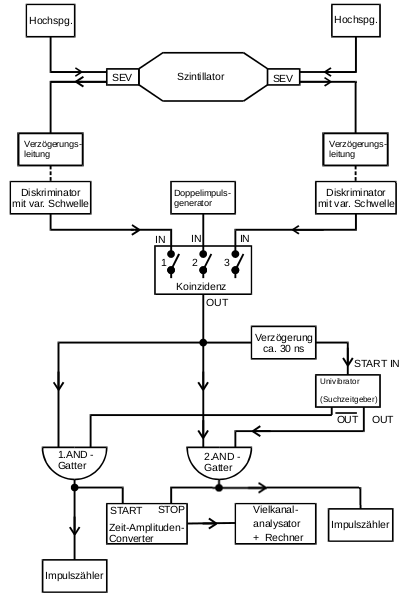
\includegraphics{Bilder/aufbau.png}
%	\label{fig:aufbau}
%\end{figure}
%
%\begin{figure}
%	\centering
%	\caption{Schematische Darstellung der Quelle zur Erzeugung radioaktiven Isotopen \cite{anleitung}.}
%	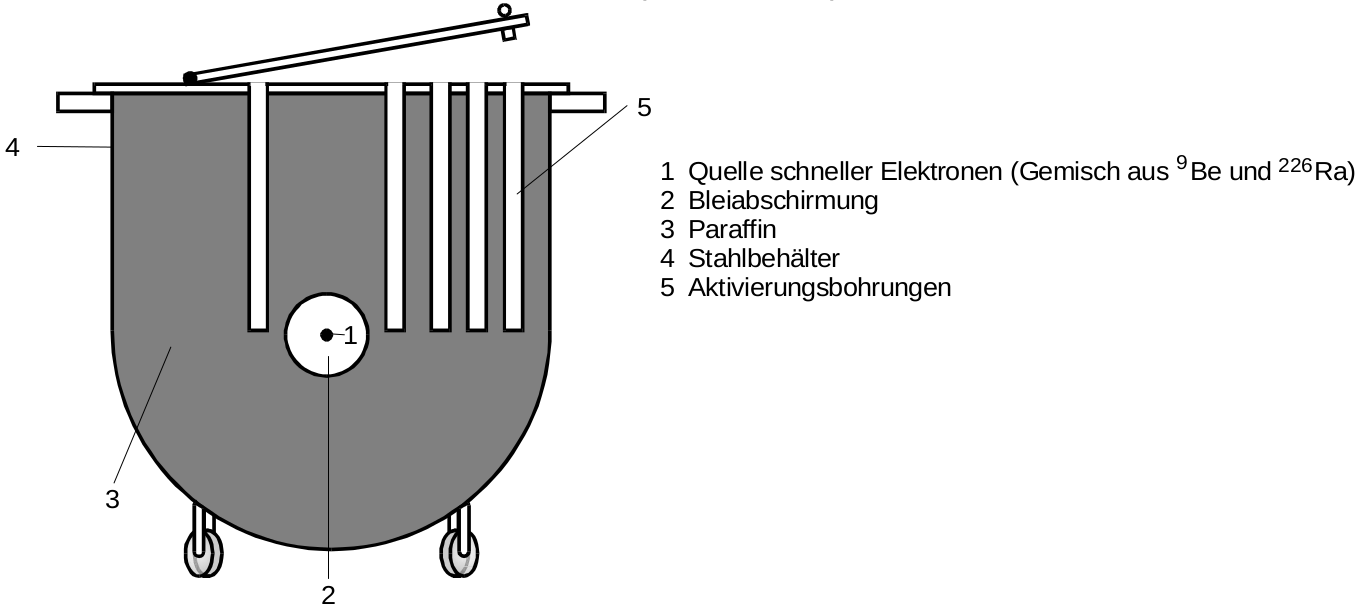
\includegraphics{content/toepfchen.png}
%	\label{fig:kochen}
%\end{figure}
%
Der Versuchsaufbau -- wie in Abbildung \ref{fig:aufbau} dargestellt -- besteht im Wesentlichen 
aus einem zerfallenden radioaktiven Isotop und einem Geiger-Müller-Zählrohr, welches die 
zerfallenden Kerne misst.
Das Geiger-Müller-Zählrohr ist entspricht einer mit Gas gefüllten Röhre. Trifft ein $\beta$-
oder $\gamma$- Teilchen auf ein Gasteilchen wird dieses ionisiert und kann aufgrund einer
anliegenden Spannung an der Röhre gemessen werden.
Dabei werden die gemessenen Zerfälle pro Messzeitintervall, welches am Zeitgeber einstellbar 
ist, an den Zählern 1 und 2 angezeigt. Nach jedem Messvorgang wird der Zähler umgeschaltet und 
der vorherige Wert auf dem aktuellen Zähler wird überschrieben. Der Versuchsaufbau ist mit
einer Blei-Abschirmung ausgestattet um die radioaktive Strahlung abzuschirmen.

Zur Erzeugung der radioaktiven Isotope wird das Objekt in Abbildung \ref{fig:kochen} verwendet.
Hierbei werden stabile Kerne mit niederenergetischen Neutronen beschossen. 
Da die Neutronen ihre Energie durch elastische Stöße an die Kerne übergeben und die maximale
Energie bei gleichen Massen der Stoßpartner erreicht wird, werden die Neutronen in einem 
Paraffinmantel gebremst, bis sie die optimale Energie besitzen.

In Abbildung \ref{fig:bild1} ist $T_2$ das wärmeabgebende und $T_1$ das wärmeaufnehmende Reservoir. Der Wärmetransport erfolgt dabei über ein reales Gas, welches beim Fluss durch $T_2$ verdampft wird, also Wärme aufnimmt
und in $T_1$ wieder verflüssigt wird und dabei seine aufgenommene Wärme wieder abgibt. \eqref{eqn:equation1}







\cite{Anleitung}
